
%% bare_conf.tex
%% V1.3
%% 2007/01/11
%% by Michael Shell
%% See:
%% http://www.michaelshell.org/
%% for current contact information.
%%
%% This is a skeleton file demonstrating the use of IEEEtran.cls
%% (requires IEEEtran.cls version 1.7 or later) with an IEEE conference paper.
%%
%% Support sites:
%% http://www.michaelshell.org/tex/ieeetran/
%% http://www.ctan.org/tex-archive/macros/latex/contrib/IEEEtran/
%% and
%% http://www.ieee.org/

%%*************************************************************************
%% Legal Notice:
%% This code is offered as-is without any warranty either expressed or
%% implied; without even the implied warranty of MERCHANTABILITY or
%% FITNESS FOR A PARTICULAR PURPOSE!
%% User assumes all risk.
%% In no event shall IEEE or any contributor to this code be liable for
%% any damages or losses, including, but not limited to, incidental,
%% consequential, or any other damages, resulting from the use or misuse
%% of any information contained here.
%%
%% All comments are the opinions of their respective authors and are not
%% necessarily endorsed by the IEEE.
%%
%% This work is distributed under the LaTeX Project Public License (LPPL)
%% ( http://www.latex-project.org/ ) version 1.3, and may be freely used,
%% distributed and modified. A copy of the LPPL, version 1.3, is included
%% in the base LaTeX documentation of all distributions of LaTeX released
%% 2003/12/01 or later.
%% Retain all contribution notices and credits.
%% ** Modified files should be clearly indicated as such, including  **
%% ** renaming them and changing author support contact information. **
%%
%% File list of work: IEEEtran.cls, IEEEtran_HOWTO.pdf, bare_adv.tex,
%%                    bare_conf.tex, bare_jrnl.tex, bare_jrnl_compsoc.tex
%%*************************************************************************

% *** Authors should verify (and, if needed, correct) their LaTeX system  ***
% *** with the testflow diagnostic prior to trusting their LaTeX platform ***
% *** with production work. IEEE's font choices can trigger bugs that do  ***
% *** not appear when using other class files.                            ***
% The testflow support page is at:
% http://www.michaelshell.org/tex/testflow/



% Note that the a4paper option is mainly intended so that authors in
% countries using A4 can easily print to A4 and see how their papers will
% look in print - the typesetting of the document will not typically be
% affected with changes in paper size (but the bottom and side margins will).
% Use the testflow package mentioned above to verify correct handling of
% both paper sizes by the user's LaTeX system.
%
% Also note that the "draftcls" or "draftclsnofoot", not "draft", option
% should be used if it is desired that the figures are to be displayed in
% draft mode.
%

\documentclass[conference]{IEEEtran}
% Add the compsoc option for Computer Society conferences.
%
% If IEEEtran.cls has not been installed into the LaTeX system files,
% manually specify the path to it like:
% \documentclass[conference]{../sty/IEEEtran}

\usepackage{color}




% Some very useful LaTeX packages include:
% (uncomment the ones you want to load)


% *** MISC UTILITY PACKAGES ***
%
%\usepackage{ifpdf}
% Heiko Oberdiek's ifpdf.sty is very useful if you need conditional
% compilation based on whether the output is pdf or dvi.
% usage:
% \ifpdf
%   % pdf code
% \else
%   % dvi code
% \fi
% The latest version of ifpdf.sty can be obtained from:
% http://www.ctan.org/tex-archive/macros/latex/contrib/oberdiek/
% Also, note that IEEEtran.cls V1.7 and later provides a builtin
% \ifCLASSINFOpdf conditional that works the same way.
% When switching from latex to pdflatex and vice-versa, the compiler may
% have to be run twice to clear warning/error messages.






% *** CITATION PACKAGES ***
%
\usepackage{cite}
% cite.sty was written by Donald Arseneau
% V1.6 and later of IEEEtran pre-defines the format of the cite.sty package
% \cite{} output to follow that of IEEE. Loading the cite package will
% result in citation numbers being automatically sorted and properly
% "compressed/ranged". e.g., [1], [9], [2], [7], [5], [6] without using
% cite.sty will become [1], [2], [5]--[7], [9] using cite.sty. cite.sty's
% \cite will automatically add leading space, if needed. Use cite.sty's
% noadjust option (cite.sty V3.8 and later) if you want to turn this off.
% cite.sty is already installed on most LaTeX systems. Be sure and use
% version 4.0 (2003-05-27) and later if using hyperref.sty. cite.sty does
% not currently provide for hyperlinked citations.
% The latest version can be obtained at:
% http://www.ctan.org/tex-archive/macros/latex/contrib/cite/
% The documentation is contained in the cite.sty file itself.






% *** GRAPHICS RELATED PACKAGES ***
%
\ifCLASSINFOpdf
  \usepackage[pdftex]{graphicx}
  % declare the path(s) where your graphic files are
  % \graphicspath{{../pdf/}{../jpeg/}}
  % and their extensions so you won't have to specify these with
  % every instance of \includegraphics
  \DeclareGraphicsExtensions{.pdf,.jpeg,.png}
\else
  % or other class option (dvipsone, dvipdf, if not using dvips). graphicx
  % will default to the driver specified in the system graphics.cfg if no
  % driver is specified.
  % \usepackage[dvips]{graphicx}
  % declare the path(s) where your graphic files are
  % \graphicspath{{../eps/}}
  % and their extensions so you won't have to specify these with
  % every instance of \includegraphics
  % \DeclareGraphicsExtensions{.eps}
\fi
% graphicx was written by David Carlisle and Sebastian Rahtz. It is
% required if you want graphics, photos, etc. graphicx.sty is already
% installed on most LaTeX systems. The latest version and documentation can
% be obtained at:
% http://www.ctan.org/tex-archive/macros/latex/required/graphics/
% Another good source of documentation is "Using Imported Graphics in
% LaTeX2e" by Keith Reckdahl which can be found as epslatex.ps or
% epslatex.pdf at: http://www.ctan.org/tex-archive/info/
%
% latex, and pdflatex in dvi mode, support graphics in encapsulated
% postscript (.eps) format. pdflatex in pdf mode supports graphics
% in .pdf, .jpeg, .png and .mps (metapost) formats. Users should ensure
% that all non-photo figures use a vector format (.eps, .pdf, .mps) and
% not a bitmapped formats (.jpeg, .png). IEEE frowns on bitmapped formats
% which can result in "jaggedy"/blurry rendering of lines and letters as
% well as large increases in file sizes.
%
% You can find documentation about the pdfTeX application at:
% http://www.tug.org/applications/pdftex





% *** MATH PACKAGES ***
%
\usepackage[cmex10]{amsmath}
% A popular package from the American Mathematical Society that provides
% many useful and powerful commands for dealing with mathematics. If using
% it, be sure to load this package with the cmex10 option to ensure that
% only type 1 fonts will utilized at all point sizes. Without this option,
% it is possible that some math symbols, particularly those within
% footnotes, will be rendered in bitmap form which will result in a
% document that can not be IEEE Xplore compliant!
%
% Also, note that the amsmath package sets \interdisplaylinepenalty to 10000
% thus preventing page breaks from occurring within multiline equations. Use:
\interdisplaylinepenalty=2500
% after loading amsmath to restore such page breaks as IEEEtran.cls normally
% does. amsmath.sty is already installed on most LaTeX systems. The latest
% version and documentation can be obtained at:
% http://www.ctan.org/tex-archive/macros/latex/required/amslatex/math/





% *** SPECIALIZED LIST PACKAGES ***
%
%\usepackage{algorithmic}
% algorithmic.sty was written by Peter Williams and Rogerio Brito.
% This package provides an algorithmic environment fo describing algorithms.
% You can use the algorithmic environment in-text or within a figure
% environment to provide for a floating algorithm. Do NOT use the algorithm
% floating environment provided by algorithm.sty (by the same authors) or
% algorithm2e.sty (by Christophe Fiorio) as IEEE does not use dedicated
% algorithm float types and packages that provide these will not provide
% correct IEEE style captions. The latest version and documentation of
% algorithmic.sty can be obtained at:
% http://www.ctan.org/tex-archive/macros/latex/contrib/algorithms/
% There is also a support site at:
% http://algorithms.berlios.de/index.html
% Also of interest may be the (relatively newer and more customizable)
% algorithmicx.sty package by Szasz Janos:
% http://www.ctan.org/tex-archive/macros/latex/contrib/algorithmicx/




% *** ALIGNMENT PACKAGES ***
%
%\usepackage{array}
% Frank Mittelbach's and David Carlisle's array.sty patches and improves
% the standard LaTeX2e array and tabular environments to provide better
% appearance and additional user controls. As the default LaTeX2e table
% generation code is lacking to the point of almost being broken with
% respect to the quality of the end results, all users are strongly
% advised to use an enhanced (at the very least that provided by array.sty)
% set of table tools. array.sty is already installed on most systems. The
% latest version and documentation can be obtained at:
% http://www.ctan.org/tex-archive/macros/latex/required/tools/


%\usepackage{mdwmath}
%\usepackage{mdwtab}
% Also highly recommended is Mark Wooding's extremely powerful MDW tools,
% especially mdwmath.sty and mdwtab.sty which are used to format equations
% and tables, respectively. The MDWtools set is already installed on most
% LaTeX systems. The lastest version and documentation is available at:
% http://www.ctan.org/tex-archive/macros/latex/contrib/mdwtools/


% IEEEtran contains the IEEEeqnarray family of commands that can be used to
% generate multiline equations as well as matrices, tables, etc., of high
% quality.


%\usepackage{eqparbox}
% Also of notable interest is Scott Pakin's eqparbox package for creating
% (automatically sized) equal width boxes - aka "natural width parboxes".
% Available at:
% http://www.ctan.org/tex-archive/macros/latex/contrib/eqparbox/





% *** SUBFIGURE PACKAGES ***
%\usepackage[tight,footnotesize]{subfigure}
% subfigure.sty was written by Steven Douglas Cochran. This package makes it
% easy to put subfigures in your figures. e.g., "Figure 1a and 1b". For IEEE
% work, it is a good idea to load it with the tight package option to reduce
% the amount of white space around the subfigures. subfigure.sty is already
% installed on most LaTeX systems. The latest version and documentation can
% be obtained at:
% http://www.ctan.org/tex-archive/obsolete/macros/latex/contrib/subfigure/
% subfigure.sty has been superceeded by subfig.sty.



%\usepackage[caption=false]{caption}
%\usepackage[font=footnotesize]{subfig}
% subfig.sty, also written by Steven Douglas Cochran, is the modern
% replacement for subfigure.sty. However, subfig.sty requires and
% automatically loads Axel Sommerfeldt's caption.sty which will override
% IEEEtran.cls handling of captions and this will result in nonIEEE style
% figure/table captions. To prevent this problem, be sure and preload
% caption.sty with its "caption=false" package option. This is will preserve
% IEEEtran.cls handing of captions. Version 1.3 (2005/06/28) and later
% (recommended due to many improvements over 1.2) of subfig.sty supports
% the caption=false option directly:
%\usepackage[caption=false,font=footnotesize]{subfig}
%
% The latest version and documentation can be obtained at:
% http://www.ctan.org/tex-archive/macros/latex/contrib/subfig/
% The latest version and documentation of caption.sty can be obtained at:
% http://www.ctan.org/tex-archive/macros/latex/contrib/caption/




% *** FLOAT PACKAGES ***
%
\usepackage{fixltx2e}
% fixltx2e, the successor to the earlier fix2col.sty, was written by
% Frank Mittelbach and David Carlisle. This package corrects a few problems
% in the LaTeX2e kernel, the most notable of which is that in current
% LaTeX2e releases, the ordering of single and double column floats is not
% guaranteed to be preserved. Thus, an unpatched LaTeX2e can allow a
% single column figure to be placed prior to an earlier double column
% figure. The latest version and documentation can be found at:
% http://www.ctan.org/tex-archive/macros/latex/base/



\usepackage{stfloats}
% stfloats.sty was written by Sigitas Tolusis. This package gives LaTeX2e
% the ability to do double column floats at the bottom of the page as well
% as the top. (e.g., "\begin{figure*}[!b]" is not normally possible in
% LaTeX2e). It also provides a command:
%\fnbelowfloat
% to enable the placement of footnotes below bottom floats (the standard
% LaTeX2e kernel puts them above bottom floats). This is an invasive package
% which rewrites many portions of the LaTeX2e float routines. It may not work
% with other packages that modify the LaTeX2e float routines. The latest
% version and documentation can be obtained at:
% http://www.ctan.org/tex-archive/macros/latex/contrib/sttools/
% Documentation is contained in the stfloats.sty comments as well as in the
% presfull.pdf file. Do not use the stfloats baselinefloat ability as IEEE
% does not allow \baselineskip to stretch. Authors submitting work to the
% IEEE should note that IEEE rarely uses double column equations and
% that authors should try to avoid such use. Do not be tempted to use the
% cuted.sty or midfloat.sty packages (also by Sigitas Tolusis) as IEEE does
% not format its papers in such ways.





% *** PDF, URL AND HYPERLINK PACKAGES ***
%
\usepackage{url}
% url.sty was written by Donald Arseneau. It provides better support for
% handling and breaking URLs. url.sty is already installed on most LaTeX
% systems. The latest version can be obtained at:
% http://www.ctan.org/tex-archive/macros/latex/contrib/misc/
% Read the url.sty source comments for usage information. Basically,
% \url{my_url_here}.





% *** Do not adjust lengths that control margins, column widths, etc. ***
% *** Do not use packages that alter fonts (such as pslatex).         ***
% There should be no need to do such things with IEEEtran.cls V1.6 and later.
% (Unless specifically asked to do so by the journal or conference you plan
% to submit to, of course. )


% correct bad hyphenation here
\hyphenation{op-tical net-works semi-conduc-tor}


\begin{document}
%
% paper title
% can use linebreaks \\ within to get better formatting as desired
\title{An Ontology Polysystem Driven Technique for Semantic Markup from Edited Documents}


% author names and affiliations
% use a multiple column layout for up to three different
% affiliations
%% \author{\IEEEauthorblockN{Evgeny Cherkashin, Polina Belykh}
%% \IEEEauthorblockA{Institute of System Dynamics\\ and Control Theory at SB RAS,\\ Irkutsk, Lermontov str., 134, 664033, Russia\\
%% Email:eugeneai\@icc.ru}
%% %\and
%% %\IEEEauthorblockN{Polina Belykh}
%% %\IEEEauthorblockA{Institute of System Dynamics\\ and Control Theory at SB RAS,\\ Irkutsk, %Lermontov str., 134, 664033, Russia}
%% \and
%% \IEEEauthorblockN{Kristina Paskal}
%% \IEEEauthorblockA{National Research\\ Irkutsk State Technical University,\\ Irkutsk, Lermontov str.,  83, 664074, Russia}}

% conference papers do not typically use \thanks and this command
% is locked out in conference mode. If really needed, such as for
% the acknowledgment of grants, issue a \IEEEoverridecommandlockouts
% after \documentclass

% for over three affiliations, or if they all won't fit within the width
% of the page, use this alternative format:
%
\author{\IEEEauthorblockN{Evgeny Cherkashin\IEEEauthorrefmark{1}\IEEEauthorrefmark{2},
Kristina Paskal\IEEEauthorrefmark{2}\IEEEauthorrefmark{3}},
\IEEEauthorblockN{Igor Bychkov\IEEEauthorrefmark{1}},
Kristina Paskal\IEEEauthorrefmark{2}  and
Polina Belykh\IEEEauthorrefmark{1}%
\IEEEauthorblockA{\IEEEauthorrefmark{1}Institute of System Dynamics and Control Theory at SB RAS, Irkutsk, Lermontov str., 134, 664033, Russia}%
\IEEEauthorblockA{\IEEEauthorrefmark{2}National Research Irkutsk State
  Technical University, Irkutsk, Lermontov str.,  83, 664074, Russia}%
\IEEEauthorblockA{\IEEEauthorrefmark{3}Irkutsk State University,
  Irkutsk, Gagarina blvd., 664003, Russia}%
}

% use for special paper notices
%\IEEEspecialpapernotice{(Invited Paper)}




% make the title area
\maketitle


\begin{abstract}
%\boldmath
  An approach to an ontology based document logical content
  representation and induction is considered. The logical layer is
  induced during content editing by means of polysystem of ontologies
  of the domain, change structure analysis, data mining and user
  interview clarifying meaning of his/her actions. The polysystem of
  ontologies are used to drive the process of user interview. As a
  result new RDF triples representing a part of the domain are
  constructed. This results in the necessity to develop document and
  content management software as knowledge acquisition systems, where
  user plays basically the role of an information source. As a testing
  ground we have chosen document preparation automation of Russian
  notary office due to a balance of structured and unstructured data
  in legal documents. The workflow of documents between offices and
  individuals can be organized as distributed social network.

\e{  A general idea of an approach to representation and induction of a
  semantic markup (logical layer) for description of the text content
  (internet sites, legal documents, and so on) is being described.
  The logical layer is generated on the base of analysis of changes
  introduced by user.  The changes of the text and the logical layer
  are analyzed.  The variant of the interpretation (e.g., error
  correction of a value or a new statement definition) of the changes
  is determined by means of user interview.  The interpretation also
  depends on the results of analysis of user behavior, e.g., patterns
  of transitions between various kinds of documents.  The theoretical
  basis of the technique is to use of a polysystem representation of
  ontologies for the domain.  The presentation is a hierarchically
  fibered structure of concepts and relations, which are mapped
  between fibers by means of interpretation relations.

  An automation of document preparation activities in a notary office
  has been chosen as a testing ground for the technologies under
  development.  The documents that are originated and used there have
  an important common property.  The documents contain information
  which is represented as structural and nonstructural data equally
  likely.
}

\end{abstract}
% IEEEtran.cls defaults to using nonbold math in the Abstract.
% This preserves the distinction between vectors and scalars. However,
% if the conference you are submitting to favors bold math in the abstract,
% then you can use LaTeX's standard command \boldmath at the very start
% of the abstract to achieve this. Many IEEE journals/conferences frown on
% math in the abstract anyway.

% no keywords




% For peer review papers, you can put extra information on the cover
% page as needed:
% \ifCLASSOPTIONpeerreview
% \begin{center} \bfseries EDICS Category: 3-BBND \end{center}
% \fi
%
% For peerreview papers, this IEEEtran command inserts a page break and
% creates the second title. It will be ignored for other modes.
\IEEEpeerreviewmaketitle



\section{Introduction}
% no \IEEEPARstart
In 2001 Tim Berners-Lee proposed a blueprint \cite{b1} of the web development that is aimed at the implementation of network services with reasonable integration of logical layer of the information presented. The information should be marked up semantically and the program agents should take advantage of the markup as the logical layer for the information consumption and processing. The blueprint is referred to as Semantic Web (SW) \cite{b1}.

One of the main problems of SW is the fact, that the regular users of the web resources are not fond of the technological aspects of SW. They are interested in their practical problems solutions. In order to involve users in SW content development, the technological aspects must be completely hidden from them. This results in the necessity to develop document and site content management software exploited within SW as knowledge acquisition systems, where user will play role of information source for a system-integrated decision-making engine.

To be more comprehensible consider a content of a legal document, which in most cases contains meaningful information for human beings relationships that is usually passed to other documents in a derivative form. This suggests an idea to develop a form of the logical layer representation in a reasonably detailed form, which can be rendered as a regular text pages by means of context"=depended (in sense of a legal document) text templates. The SW approach could supplement the idea with data formats and technologies of their storage and processing. SW represents logical layer as a network graph of notions and relations between the notions. For example, individuals mentioned in a legal document relate to the document as “parts"=whole”, unless to speak even more explicitly in a context of the meaningful information.

At present most of the use cases of domain ontology models are refining search results. Automatic procedures of ontology extraction from the documents are based on crawling documents in a warehouse, data mining procedures on the text bodies and metadata attributes of the documents. Simple observation of the human behavior in the process of a document preparation will result in the confidence that meaningful parts of the document, which are usually expressed with the logical layer, are located at the points of document changes. Hence, a programming system automating a document preparation should track the changes and analyze them in the time space to extract ontology data, i.e., data (a"=box and corresp. relations) and knowledge (t"=box with corresp. relations).

The logical layer is induced during content edition by means of data mining and user interview. The context of the knowledge acquisition consists of a polysystem of ontologies describing the domain, the source document (its textual representation and the existing logical structure), its list of modifications in a transaction, user's action history and answers to the interview questions clarifying meaning of his/her actions and properties of the relations constructed. As a result new or modified triples <subject, relation, object> representing the domain are constructed. Collected triple data, metadata and knowledge of the logical layer can also be crawled on a regular basis to figure out patterns and functional relations between attributes (objects). In the last case a relational table could be induced to rise the efficiently of data storage and processing.

The present trends of internet information system development show that the systems become a web services and are oriented to support social networks \cite{b3}. The data flow processing here in most cases is input, storage, filtering and transmitting data, i.e., the social networks integrate rather than aggregate data, e.g., to produce reports. Hence, the usage of special design techniques for the middleware layer of the software, such as object-oriented design, is not a significant advantage. Social network are interconnected with common protocols and data structures, also in the social network environment

\begin{IEEEitemize}[\IEEEsetlabelwidth{Z}]
\item there are no predominant common task to be solved with all the agents (computer and human);
\item each agent solves its special task, so the agent API’s and supported data format must be strongly standardized;
\item human users of the social network do most of the aggregation tasks personally including subconscious joint processing of unstructured and semantic information.
\end{IEEEitemize}

In this paper, we continue the development of the approach to document and site content management and integration [-2-], where human users play a role of data sources in the process of semantic data markup formation of the document content.

As a testing ground, we have chosen document preparation automation of a Russian notary office. Most of all operations over documents can be expressed as textual and logical layer changes, for example, data of the logical layer are copied from one document to another; sometimes roles of individuals mentioned in the documents are alternated; database collects client data for further reuse (lookup), \emph{etc}.

\section{Logical Markup Procedure of the Document Content}

The RDF standard describes informational resources as triples <subject, relation, object> in a context. The set of triples forms a graph (network) of data and relations reflecting knowledge. It is convenient to divide graphs to subgraphs and construct their hierarchic complexes \cite{b4}, resulting a hierarchy of contexts. In a general case, a context affects the interpretation of its set of triples. For example, family name and passport data are presented as texts in different parts of the document, but related to the single person in the context defined by the document.

The rendering engine we considered in [-2-]. In this approach, all the template data for document rendering is also stored in the ontology graph. We also represent the views and algorithms implementing controllers in the sense of MVC (Model View Controller) technique with triples \cite{b5}. The content of the document from a general view is a tree, where almost each node is both a subject and an object of their corresponding relations (fig.1). The exceptions are the root node\,: it plays only the role of subject, and the leaf nodes that are objects only. In the higher level hierarchies, e.g. in a tree of the documents in a warehouse, the root node is an object node as well (it is referred from a record of the warehouse).

One of the key points of the research is semantic document markup techniques adaptation to the process of document editing. We suppose that a document body change, in a regular case, affects the meaning of the document, hence, alters its logical layer. Examples of the modifications are the elementary error correction, a field value change (an object of a triple), paragraph text editing that might imply its origin template correction. Each change also might result in a new triple relation construction between context subjects and old/new object value. The text change analysis is aimed at data and knowledge acquisition, where the content management system plays an active role, and user is a source of complementary information.

The semantic layer enrichment is carried on in an environment containing logic information thanks to document is already supplied with a logical layer. The source data for an acquisition step is as follows\,: a) the source version of the document, b) a text modification expressed in diff format \cite{b9}; c) user answers to the question asked by the system, which refine the semantics and structure of the modifications; d) user actions preceding the modification. If the modification corresponds to a value of an object of a triple then the modification means either error correction (subject is not changed) or creation of a new subject if user copied the document previously. Creation of a new document implies filling in a number of triples with new values representing a new subject (RDF resource) of the document.

If a field or a text is partially modified this can be interpreted as:
\begin{itemize}
\item again, an error correction without document meaning change;
\item a refinement of the logical structure of subject, extraction of a relation and an object; this corresponds to a new triple connecting the subject to the new object (changed value); the user must choose the subject of the new triple.
\end{itemize}

The new subject is chosen from a tree of all the subjects of the edited document. After the choice is made, a list of all available relation is constructed from all known relation of the subject, its class and parent classes. User must choose one relation to form the triple. In the case, when the list contains no desired relation, a new one must be defined. New relation is always a subclass of one that already exists in the system, which is also chosen from the list. New relations defined by inexperienced user must be periodically analyzed by knowledge engineers to get rid of semantic inaccuracy, contradictions, redundancy to the equivalents, and be, hence, refactored.

If a value of a triple is removed, then the triple is being removed too. The situation is acceptable if the minimal structural and semantic completeness of all the subjects of the documents are hold, otherwise either the user delete action is prohibited or the chain recursive deletion of the subjects is initiated. To control this behavior each subject class have to be accompanied with a list of minimal valuable triplets that define the basis of the subject meaning. Partial text removal, if it is not an error correction, is processed analogously to modification, with removed part being the object value. Addition of characters to text is an action similar to modification, i.e., in a general case a new triple is constructed.

Addition of a triple might result in extending the document with new subjects and relations. For example, let construct a new tripartite agreement from an existing bilateral one. In new contract a third individual appeared, so the addition of a new family name of the individual results in construction of a subject for the individual, filling in the necessary triples, as well as definition of a new relation between document and the subject as a subclass of structuralElement relation.

\section{Theoretical Generalization of the Acquisition Process}

The above described approach is a stepwise implementation of polysystem analysis and synthesis \cite{father} (PSAS) procedure. This is a general procedure for system analysis of domains. The essence of the approach is that domain and any its object or process can be fibrated and represent it in multidimensional space of fiber-coordinates. This approach is used in control problem solution, decomposition, analysis and synthesis of complex systems. In comparison to system approach, where the principle of interconnection of the elements is fundamental, polysystem analysis assumes the hypothesis of fibration, i.e., it supposes a possibility of representation of the object under investigation as disjoint subsets, thus, mutually unbound fibers (subdomains). So, in a generalized insight a polysystem is a system itself, and polysystem analysis is a new form of system analysis.

The application of the PSAS to the process of data and knowledge acquisition in the documents expressed as simultaneus polysystem fibering the domain in various coordinate systems (aspects) as follows\,: structural organization of a document (mereological aspect), expressing domain of activity area, hierarchical inheritance of various kind of documents (domain system concept inheritance), people and organization relationship, deontic logic representation of the document meaning, etc.

According to PSAS \cite{father} each concept of an aspect should be presented (via interpretation morphisms) in all other fibers as well as its relationships with adjacent concepts. Theoretically, for each of the fibers, a complete theory of the domain can be constructed. Each theory differ by their fundamental concept, but they are similar each other via concept substitution (an interpretation); this allows us to induce new axiomatic theories of domains in the image and likeness of the known ones. Each system domain (fiber) of knowledge fibrates multiply and sequentially, giving raise of the polysystem of representation of an object under investigation. All the system theories are combined in the unified model describing the domain and the object.

In our case we defined the procedure of triples acquisition as an instance of the fibration procedure. The obtained classes of documents, people and other objects are the concept of a PSAS theory of an aspect. Having established new class or new relation between two classes, the concept or relation should be reflected as a substituted (interpreted with) one in other ontologies (e.g., mereological one). In a general case we must also produce the definitions for the notions in those ontologies.

Each of new concept (a class) as we described in the previous section is to be inherited from a parent class, thus, it can be interpreted in other ontologies as either a concept that corresponds to the parent class or to a new inherited class. This case the user interview also organized to obtain a description of the class and the relation.

Thus, the usage of the PSAS allows us to partially deal with the completeness (As \ldots{} \cite{sergey}) and consistency (by testing an ontology and morphing the results to other ones) of the ontological theories under construction.

\subsection{Utilizing Polysystem of Ontologies in User Interview}
As it was mentioned above any studied and modeled domain can be fibrated and represented as a polysystem of notions, objects and their relationships. The polysystem from a general point of view is a set of disjoint layers. Each layer contains a system of concepts, individual objects and corresponding relationships between them. In a fibrated polysystem, concepts belonging to a layer are morfed (mapped) into concepts in other layers via concept interpretation of one layer (projection, theory, science, domain) into concepts of other layer. All the concepts are interpreted by concepts of the abstract system layer. The interpretation feature of polysystem layers could be used to drive user interview dialog on the base of an inference by analogy represented as movement along relations and morphs in the polysystem of ontologies.

Consider simple family relationships in fig.~\ref{OPSA}, where most of the obvious relations are hidden to make the figure more readable. There are four main layers in the figure, which model corresponding aspects of Bob's family: layer 1 represents the family itself, it is the only layer having a-box entities; layer 2 represent main roles of individuals in a family; layer 3 shows genders as two opposites; and later 4 corresponds to mereological metomodel ``whole--parts''.

Let's construct a list of questions to determine a role of Jul in Bob's family. It is supposed we know only that Jul is a female. To put Jul in layer 1, we must ask a general question: ``Is Jul a part of Bob's family?'' The question is constructed according to a following intuitive inference. All relations between a family and its members are kinds of ``partOf:'' relation from layer 4. This fact is shown as an arrow from relation hasFather: of Layer 2 to ``partOf:'' of Layer 4, other four arrows are hidden. So, in order to determine the fact that Jul is a member of Bob's family, it is sufficient to ask ``Is Jul partOf: Bob's-family?''. The identifier of the example family is devised from the tradition to name families after their master of housekeeping (MOH) person, that is denoted by arrow from individual Bob (layer 1) to concept MOH (layer 2).

If user answered positively (Jul is a part of the family), then we must refine her role, as partOf: is not a role allowed to be used in layer 1. Jul is a female (by definition), so she cannot be father and son. If she is, she must be male, but it is not as male and female are formally opposite concepts. If multiplicity of relations in the layer are defined, then we will also know, that the family already has mother. The only possible choice is Jul is daughter, resulting an another general question:''Is Jul daughter?'' If the answer to the second question is also positive, finally a new triple constructed <Bob's-family hasDaughter: Jul>.

If, e.g., gender of Jul is unknown, then the second question is constructed as a special question ``What role has Jul in Bob's family?'' and a list of two possible answers is shown: ``hasDaughter:'' and ``hasSon:''. Or it can be constructed as an alternative question ``Is Jul plays hasDaughter: or hasSon: role in the family?'', but in this case the sentence is more weird with respect to English.

\begin{figure}
\centering\sf
\def\svgwidth{0.9\linewidth}
\input{layer.pdf_tex}
\caption{An  Usage Example of an Ontology Polysystem}
\label{OPSA}
\end{figure}

(HERE: a generalizing resume paragraph needed.)

(About polysystem of ontologies).

(procedure of fibration)

(procedure of completeness reconstruction): (About mapping via functors).

(Induction of notions, suppositions of fibrations).

(wikipedia and Google search systems).

(!! Systems of complexes. !!)

\section{An Office Usage of the Technique}

One of the applications of the technology under development is document preparation automation of a notary office. Notary office in Russia generate vast amount of printed documents. The documents contain both formalized and unformalized data in a balance reasonable for our study. For example, formalized data are the passport data of individuals, registration data of vehicles. Data of this kind are passed from one document to other documents mostly sturcturized and unchanged, raising a bindles of related documents. The document content structure significantly depends on entry fields’ data filled in: form of notary signature field depends on legal capacities of the individuals mentioned in the main document body. At present templates of the documents are prepared by a programming engineer collaborating with a professional secretary and verified by supervising notary. Unformalized data are various enumerations of legal empowerments of the individuals, article codes, and explanatory text.

Application of the semantic approach to the logical layer representation of the notary document content is aimed at involvement of the secretaries (people with low engineering skills) into the processes of the document instances preparation from the existing templates and into the development of the templates and constructing their hierarchical arrangement.

Logical layer of a notary document consists of hierarchy of subjects. The subjects relate to each other on various abstraction levels, e.g., in a letter of attorney there are at least two individuals, the first one is principal, and the second one is trusted (proxy). For each individual passport, data and place of residence are defined. The letter can contain other person data, e.g., for partially capable children. All the individuals are in explicit relation to the document. The triples <letatt998 containsPrincipal indiv\_78> and <letatt998 containsProxy indiv\_79> could define a principal and proxy to the document. The mentioned relations are specifications of abstract hasIndividual and structuralElement relations. This multilevel approach allows us visually represent hierarchical structures of the document, having interpreted the relations as structural elements, and in the same time to associate individuals with other roles in new documents, swap roles during editing. The swap function is implemented as user interface widget, which recognizes certain subject-to-subject relation patterns in the document body and interprets semantics of the relations as possible action. A general graph structure of the abstract level of a notary office automation ontology is drawn in fig.~\ref{notaryontology}.

[The flexibility and minimum resources and administration requirements criteria are of very importance to choosing database providing information resources storage as triples. The database management systems as DB2, Oracle and SQL Server cannot fulfill requirements because after running the operation is performed as a separate process. Also application and DBMS interaction should be implemented through interprocess communication form.

Solution to these problems is achieved by using the built-in database management systems that provide communication with the application at the same level of address space. This allows the application based on the built-in database to be efficient and autonomous.

Kyoto Cabinet is a library of routines for managing a database. The database is a simple data file containing records, each is a pair of a key and a value. Every key and value is serial bytes with variable length. Both binary data and character string can be used as a key and a value. Each key must be unique within a database. There is neither concept of data tables nor data types. Records are organized in hash table or B+ tree. \cite{b1}

Availability of funds to work with triplets described in the standard RDF is an advantage database management system Kyoto Cabinet over other embedded systems is. In this case the developer does not need to spend time on design and implementation of the data model so that its performance on this task is increased.

1.	Kyoto Cabinet. URL: http://fallabs.com/kyotocabinet/ (дата обращения: 20.02.2014).]

%\subsubsection{Subsubsection Heading Here}
%Subsubsection text here.




% An example of a floating figure using the graphicx package.
% Note that \label must occur AFTER (or within) \caption.
% For figures, \caption should occur after the \includegraphics.
% Note that IEEEtran v1.7 and later has special internal code that
% is designed to preserve the operation of \label within \caption
% even when the captionsoff option is in effect. However, because
% of issues like this, it may be the safest practice to put all your
% \label just after \caption rather than within \caption{}.
%
% Reminder: the "draftcls" or "draftclsnofoot", not "draft", class
% option should be used if it is desired that the figures are to be
% displayed while in draft mode.
%
\begin{figure}[!t]
\centering
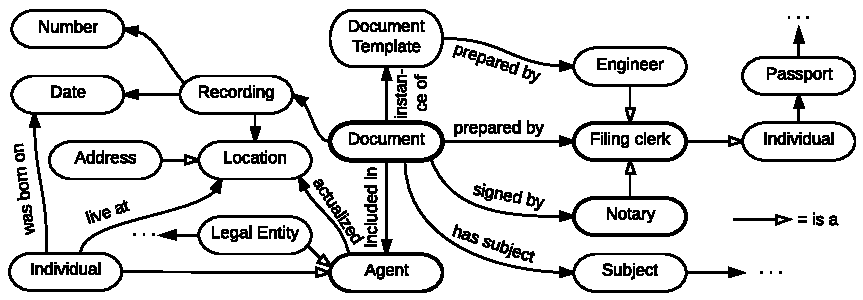
\includegraphics[width=\linewidth]{DocumentOntology-en.pdf}
% where an .eps filename suffix will be assumed under latex,
% and a .pdf suffix will be assumed for pdflatex; or what has been declared
% via \DeclareGraphicsExtensions.
\caption{An upper layer of notary office ontology}
\label{notaryontology}
\end{figure}

% Note that IEEE typically puts floats only at the top, even when this
% results in a large percentage of a column being occupied by floats.


% An example of a double column floating figure using two subfigures.
% (The subfig.sty package must be loaded for this to work.)
% The subfigure \label commands are set within each subfloat command, the
% \label for the overall figure must come after \caption.
% \hfil must be used as a separator to get equal spacing.
% The subfigure.sty package works much the same way, except \subfigure is
% used instead of \subfloat.
%
%\begin{figure*}[!t]
%\centerline{\subfloat[Case I]\includegraphics[width=2.5in]{subfigcase1}%
%\label{fig_first_case}}
%\hfil
%\subfloat[Case II]{\includegraphics[width=2.5in]{subfigcase2}%
%\label{fig_second_case}}}
%\caption{Simulation results}
%\label{fig_sim}
%\end{figure*}
%
% Note that often IEEE papers with subfigures do not employ subfigure
% captions (using the optional argument to \subfloat), but instead will
% reference/describe all of them (a), (b), etc., within the main caption.


% An example of a floating table. Note that, for IEEE style tables, the
% \caption command should come BEFORE the table. Table text will default to
% \footnotesize as IEEE normally uses this smaller font for tables.
% The \label must come after \caption as always.
%
%\begin{table}[!t]
%% increase table row spacing, adjust to taste
%\renewcommand{\arraystretch}{1.3}
% if using array.sty, it might be a good idea to tweak the value of
% \extrarowheight as needed to properly center the text within the cells
%\caption{An Example of a Table}
%\label{table_example}
%\centering
%% Some packages, such as MDW tools, offer better commands for making tables
%% than the plain LaTeX2e tabular which is used here.
%\begin{tabular}{|c||c|}
%\hline
%One & Two\\
%\hline
%Three & Four\\
%\hline
%\end{tabular}
%\end{table}


% Note that IEEE does not put floats in the very first column - or typically
% anywhere on the first page for that matter. Also, in-text middle ("here")
% positioning is not used. Most IEEE journals/conferences use top floats
% exclusively. Note that, LaTeX2e, unlike IEEE journals/conferences, places
% footnotes above bottom floats. This can be corrected via the \fnbelowfloat
% command of the stfloats package.



\section{Conclusion}
An approach to representation of logical layer of a document based on RDF (Resource Description Framework) is proposed. The approach allows us to formalize the structure and semantic relation of the document, and also store data to render the document as HTML-page in the same data format - RDF. XML and RDF allow us to join logical and presentation aspects of the document within the same storage engine. The engine stores data as an onology, i.e., set of triples <subject, relation, object>. A technique for HTML-rendering from the logical layer is described. The resulting document will contain the logical layer as a RDFa markup. The generated RDFa-markup is used at client side by web-browser for control of WYSIWYG-editing of the document. Text elements are modified with special widgets appearing in the user interface on an mouse event. A technique for organization of an interactive process of logical layer forming of the document content on the base of modifications analysis of the document content introduced by user. An example of application of the technologies under development in a notary office is presented. Thus, we shown that RDF format mixed with XML allows us to represent logical layer of meaningful information of a document, as well as sharing common data between documents.

On the base of the technology a network of document data exchange can be devised. The security of the document transmission can be provided as off-line data streams: each physical document is accompanied with its bar- or QR-code encoding the corresponding RDF-data of the transferred document. This can result in a semantic network analogous to nowadays social networks.

A part of the paper devoted to consideration of organizational problems, such as involving knowledge engineers in a refinement process of generated parts of the ontologies; partial automatic ontology verification; implementing secure ways of personal data transfer and processing. The properties of the document exchange network will be similar to social networks, and, probably, can be further developed and investigated the same way.



% conference papers do not normally have an appendix


% use section* for acknowledgement
\section*{Acknowledgment}
The research is carried on under support of Integration multidisciplinary project of Siberian Branch of Russian Academy of Sciences N 17 “Development of services and infrastructure of scientific spatial data for supporting complex multidisciplinary scientific research of Baikal nature territory”.

%The authors would like to thank...





% trigger a \newpage just before the given reference
% number - used to balance the columns on the last page
% adjust value as needed - may need to be readjusted if
% the document is modified later
%\IEEEtriggeratref{8}
% The "triggered" command can be changed if desired:
%\IEEEtriggercmd{\enlargethispage{-5in}}

% references section

% can use a bibliography generated by BibTeX as a .bbl file
% BibTeX documentation can be easily obtained at:
% http://www.ctan.org/tex-archive/biblio/bibtex/contrib/doc/
% The IEEEtran BibTeX style support page is at:
% http://www.michaelshell.org/tex/ieeetran/bibtex/
%\bibliographystyle{IEEEtran}
% argument is your BibTeX string definitions and bibliography database(s)
%\bibliography{IEEEabrv,../bib/paper}
%
% <OR> manually copy in the resultant .bbl file
% set second argument of \begin to the number of references
% (used to reserve space for the reference number labels box)
\begin{thebibliography}{11}

\bibitem{IEEEhowto:kopka}
H.~Kopka and P.~W. Daly, \emph{A Guide to \LaTeX}, 3rd~ed.\hskip 1em plus
  0.5em minus 0.4em\relax Harlow, England: Addison-Wesley, 1999.

\bibitem{TBL2001} T. Berners-Lee, J. Hendler and O. Lissila. \emph{The Semantic Web A new form of Web content that is meaningful to computers will unleash a revolution of new possibilities.}\hskip 1em plus 0.5em minus 0.4em\relax  Scientific American, May 17, 2001, pp.1-18. URL: http://sciam.com/article.cfm?articleID=00048144-10D2-1C70-84A9809EC588EF21. (access date: 05.09.2013).
\bibitem{}
Social network - Wikipedia, the free encyclopedia. URL: \url{http://en.wikipedia.org/wiki/Social_network} (access date: 20.08.2013).
\bibitem{}
Chameleon – Chameleon 2.10 documentation. \url{http://chameleon.readthedocs.org/en/latest/} (access date:  20.08.2013).
\bibitem{}
Virtuoso Open-Source Edition URL: \url{http://virtuoso.openlinksw.com/dataspace/doc/dav/wiki/Main/} (access date: 30.05.2013).
\bibitem{}
PIZZA Protege OWL tutorial at Manchester (School of Computer Science - The University of Manchester)  URL:\url{http://owl.cs.manchester.ac.uk/tutorials/protegeowltutorial/} (access date: 20.09.2013).
\bibitem{}
SWI-Prolog's home. URL: \url{http://www.swi-prolog.org/} (access date: 20.08.2013).
\bibitem{}
The Protégé Ontology Editor and Knowledge Acquisition System. URL: \url{http://protege.stanford.edu/} (access date: 20.08.2013).
Semantic MediaWiki. URL: \url{http://semantic-mediawiki.org/} (access date: 20.08.2013).
\bibitem{}
N.Heino, S.Tramp, N.Heino, S.Auer. Managing Web Content using Linked Data Principles – Combining semantic structure with dynamic content syndication. Computer Software and Applications Conference (COMPSAC), 2011 IEEE 35th Annual. pp. 245 - 250. URL:\url{http://svn.aksw.org/papers/2011/COMPSAC_lod2.eu/public.pdf} (access date: 30.05.2013).
\bibitem{}
Cherkashin E.A., Paramonov V.V., et al, Model Driven Architecture is a Complex System, E-Society Journal Research and Applications. Volume 2, Number 2, 2011, pp. 15-23.
\bibitem{}
Father


\end{thebibliography}




% that's all folks
\end{document}
